\section{Theorie}
\label{sec:Theorie}

\subsection{Grundlagen}                      
\label{sec:grundlagen}

\begin{figure}[H]
    \centering
    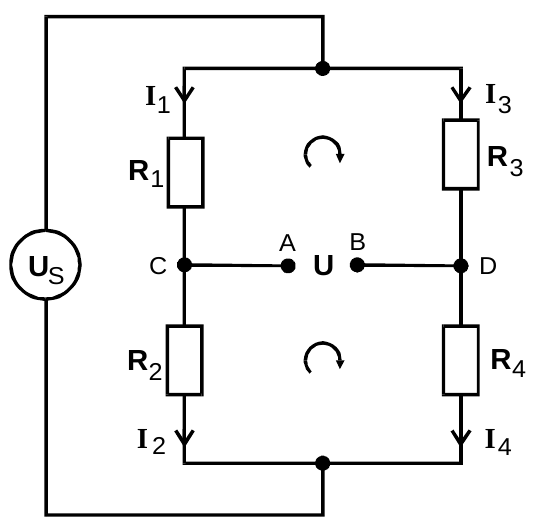
\includegraphics[scale=0.4]{pictures/1-allg.png}
    \caption{Prinzip einer Brückenschaltung}
    \label{fig:allg}
\end{figure}

\subsection{Wheatstone'sche Brückenschaltung}
\label{sec:wheatstone}

\begin{figure}[H]
    \centering
    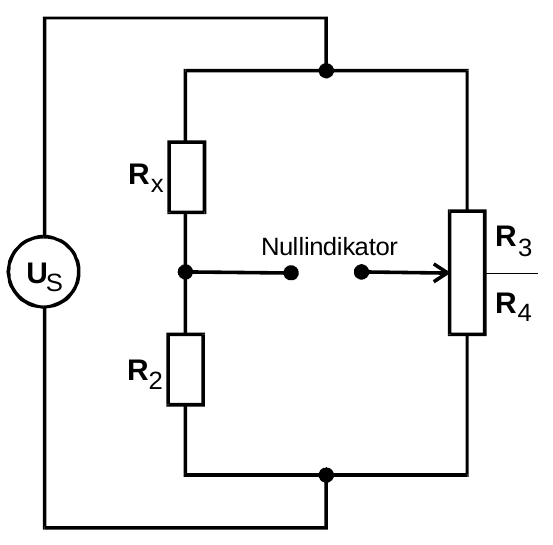
\includegraphics[scale=0.4]{pictures/2-wheatstone.png}
    \caption{Wheatstone'sche Brückenschaltung}
    \label{fig:wheatstone}
\end{figure}

\subsection{Kapazitätsmessbrücke}            
\label{sec:Cbrücke}

\begin{figure}[H]
    \centering
    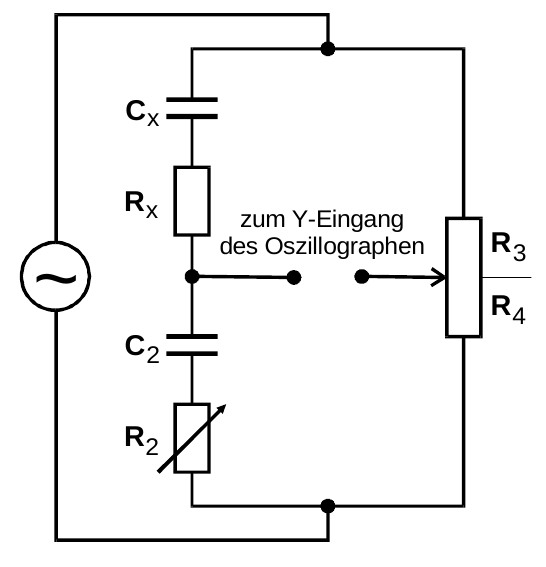
\includegraphics[scale=0.4]{pictures/3-C.png}
    \caption{Kapazitätsmessbrücke für reale Kondensatoren}
    \label{fig:Cbrücke}
\end{figure}

\subsection{Induktivitätsmessbrücke}         
\label{sec:Lbrücke}

\begin{figure}[H]
    \centering
    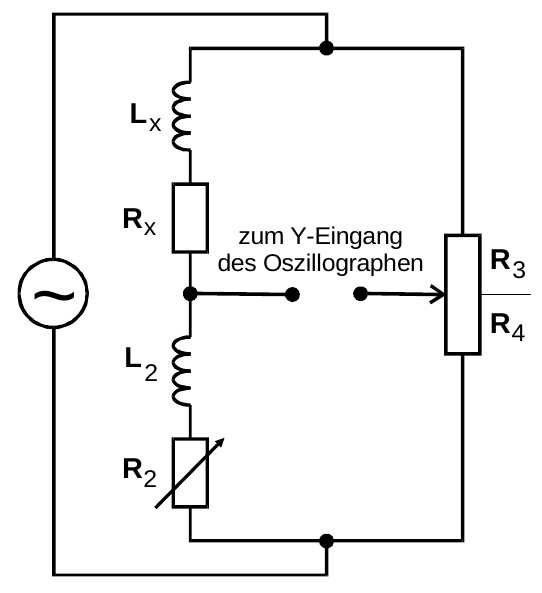
\includegraphics[scale=0.4]{pictures/4-L.png}
    \caption{Induktivitätsmessbrücke für reale Induktivitäten}
    \label{fig:Lbrücke}
\end{figure}

\subsection{Maxwell-Brücke}                  
\label{sec:maxwell}

\begin{figure}[H]
    \centering
    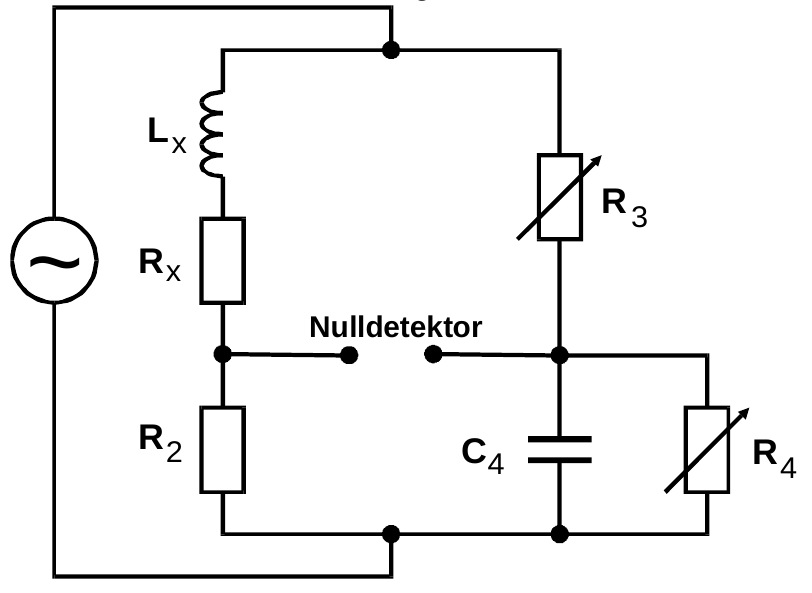
\includegraphics[scale=0.4]{pictures/5-maxwell.png}
    \caption{Maxwell-Brücke für reale Induktivitäten}
    \label{fig:maxwell}
\end{figure}

\subsection{Wien-Robinson-Brücke}             
\label{sec:wien-robinson}

\begin{figure}[H]
    \centering
    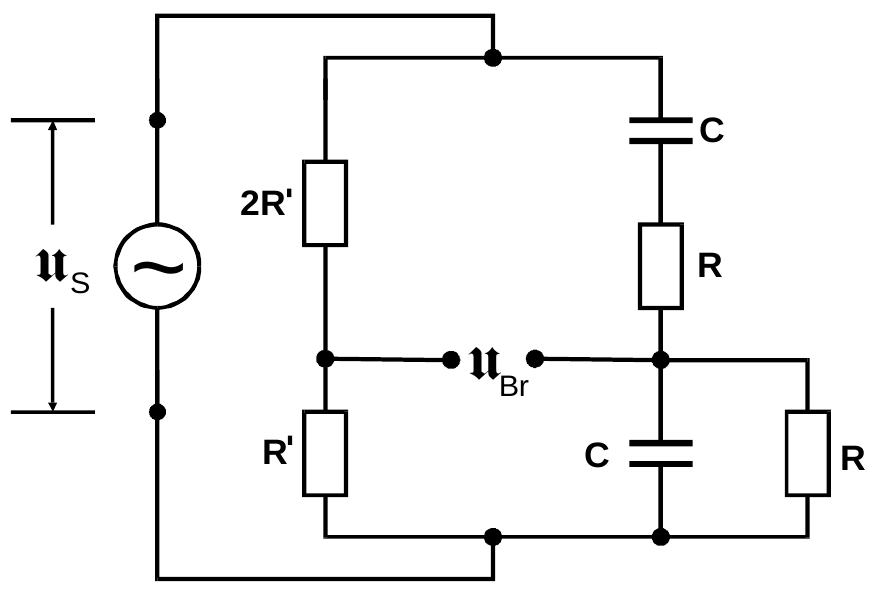
\includegraphics[scale=0.4]{pictures/6-wien-robinson.png}
    \caption{Wien-Robinson-Brücke}
    \label{fig:wien-robinson}
\end{figure}

\subsection{TT-Brücke}                       
\label{sec:TT}

\begin{figure}[H]
    \centering
    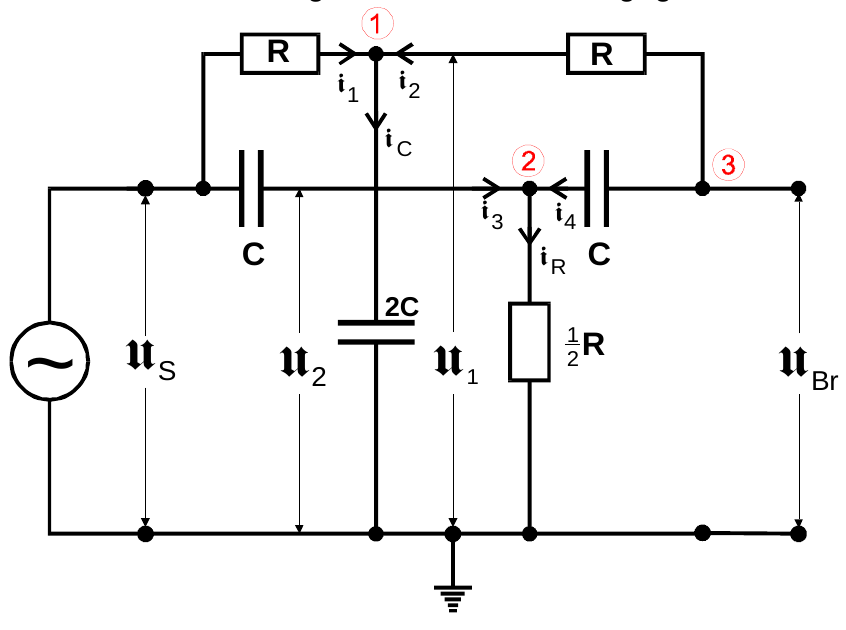
\includegraphics[scale=0.4]{pictures/7-TT.png}
    \caption{TT-Brücke}
    \label{fig:TT}
\end{figure}
